The high atmosphere can be seen
as given in Fig.~\ref{Titan_high_atm}, taken
from \cite{Waite07}.

\begin{figure}
\centering
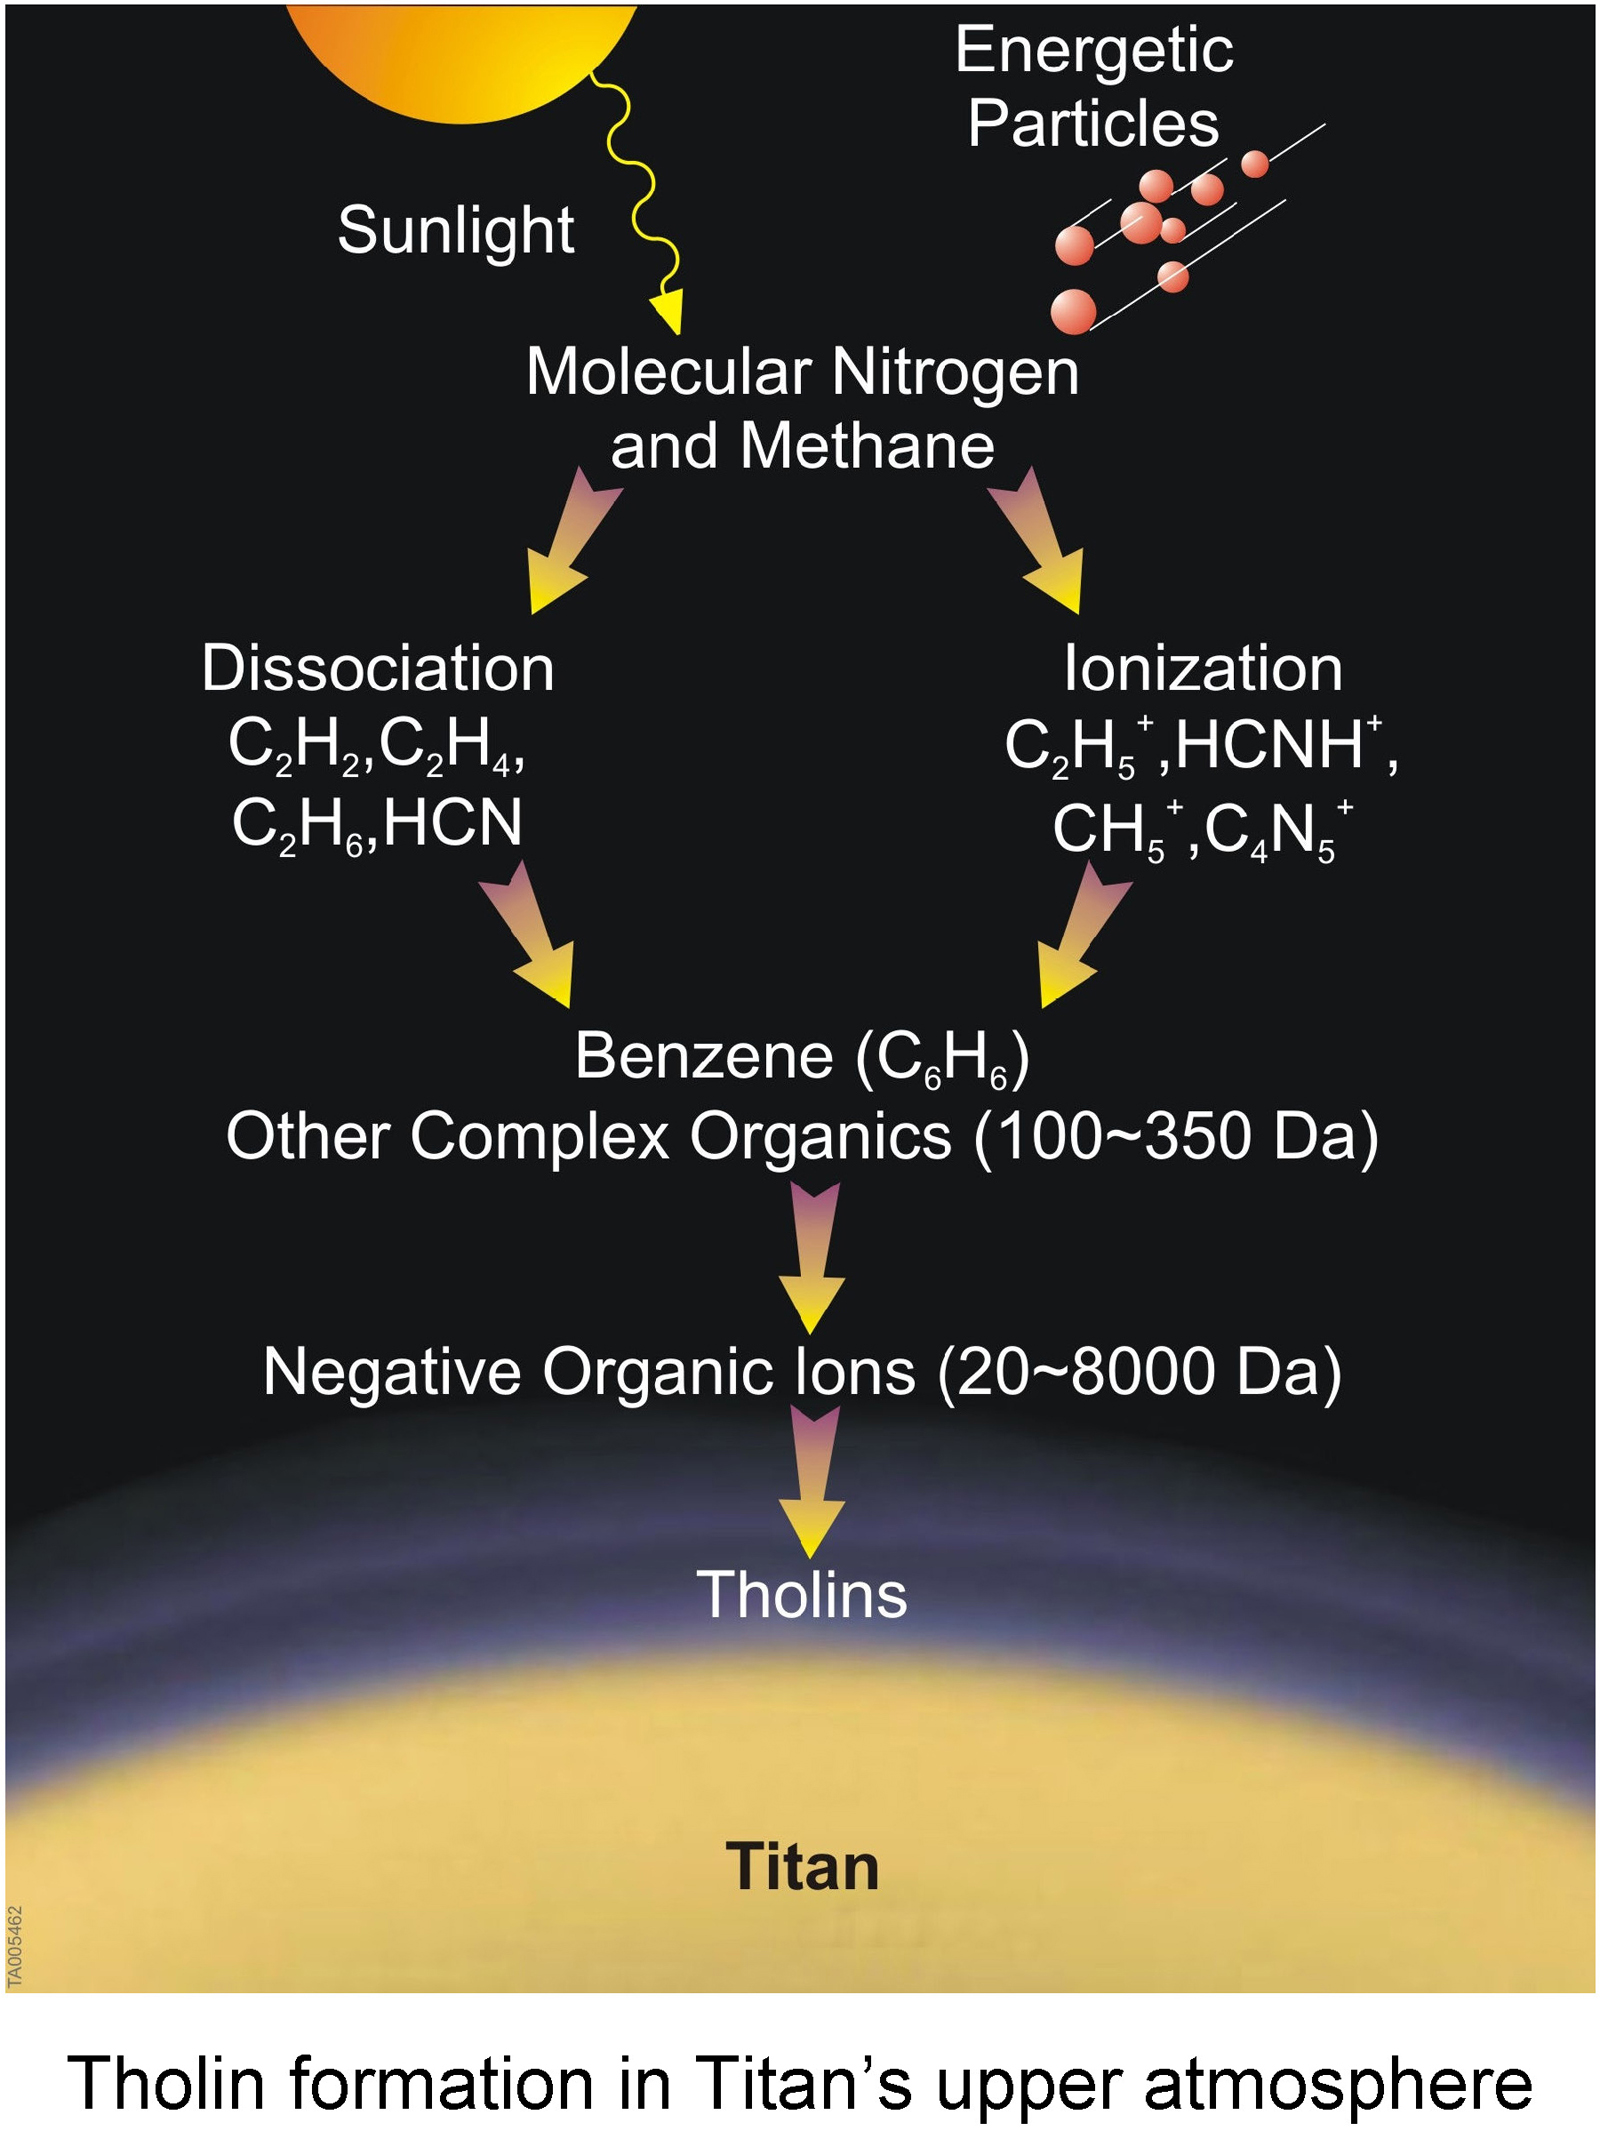
\includegraphics{Titan_Waite07}
\caption{\label{Titan_high_atm}Physical processes in the high
atmosphere of Titan}
\end{figure}

To investigate, there were flybys. A flyby dataset contains:
\begin{itemize}
\item A zenith angle of approach;
\item a sub-solar latitude;
\item a lower boundary total density;
\item a lower boundary temperature;
\item an iso-thermal temperature;
\item an eddy coefficient;
\item mixing ratios for a composition.
\end{itemize}
